%!TEX program = lualatex
% img.tex
\documentclass{article}

\usepackage{emoji}
\usepackage{graphicx}
\usepackage{float}
\usepackage{subfig}

\title{Image \emoji{book}}
\author{oeyoews}
\date{2022/08/09}

\graphicspath{{img/}}
\begin{document}

\maketitle

\section{\emoji{book} Images}
\label{sec:img}

\begin{table}
\begin{tabular}{|c|c|c|}\hline
	
\includegraphics[width=0.3\textwidth]{tw-tada} & 
\includegraphics[width=0.3\textwidth]{tw-tada} & 
\includegraphics[width=0.3\textwidth]{latex} \\\hline
\end{tabular}
\end{table}

\begin{figure}[htpb]
  \centering
  
\includegraphics{island}
  \caption{island}
  \label{fig:island}
\end{figure}

\begin{figure}[htpb]
  \centering
  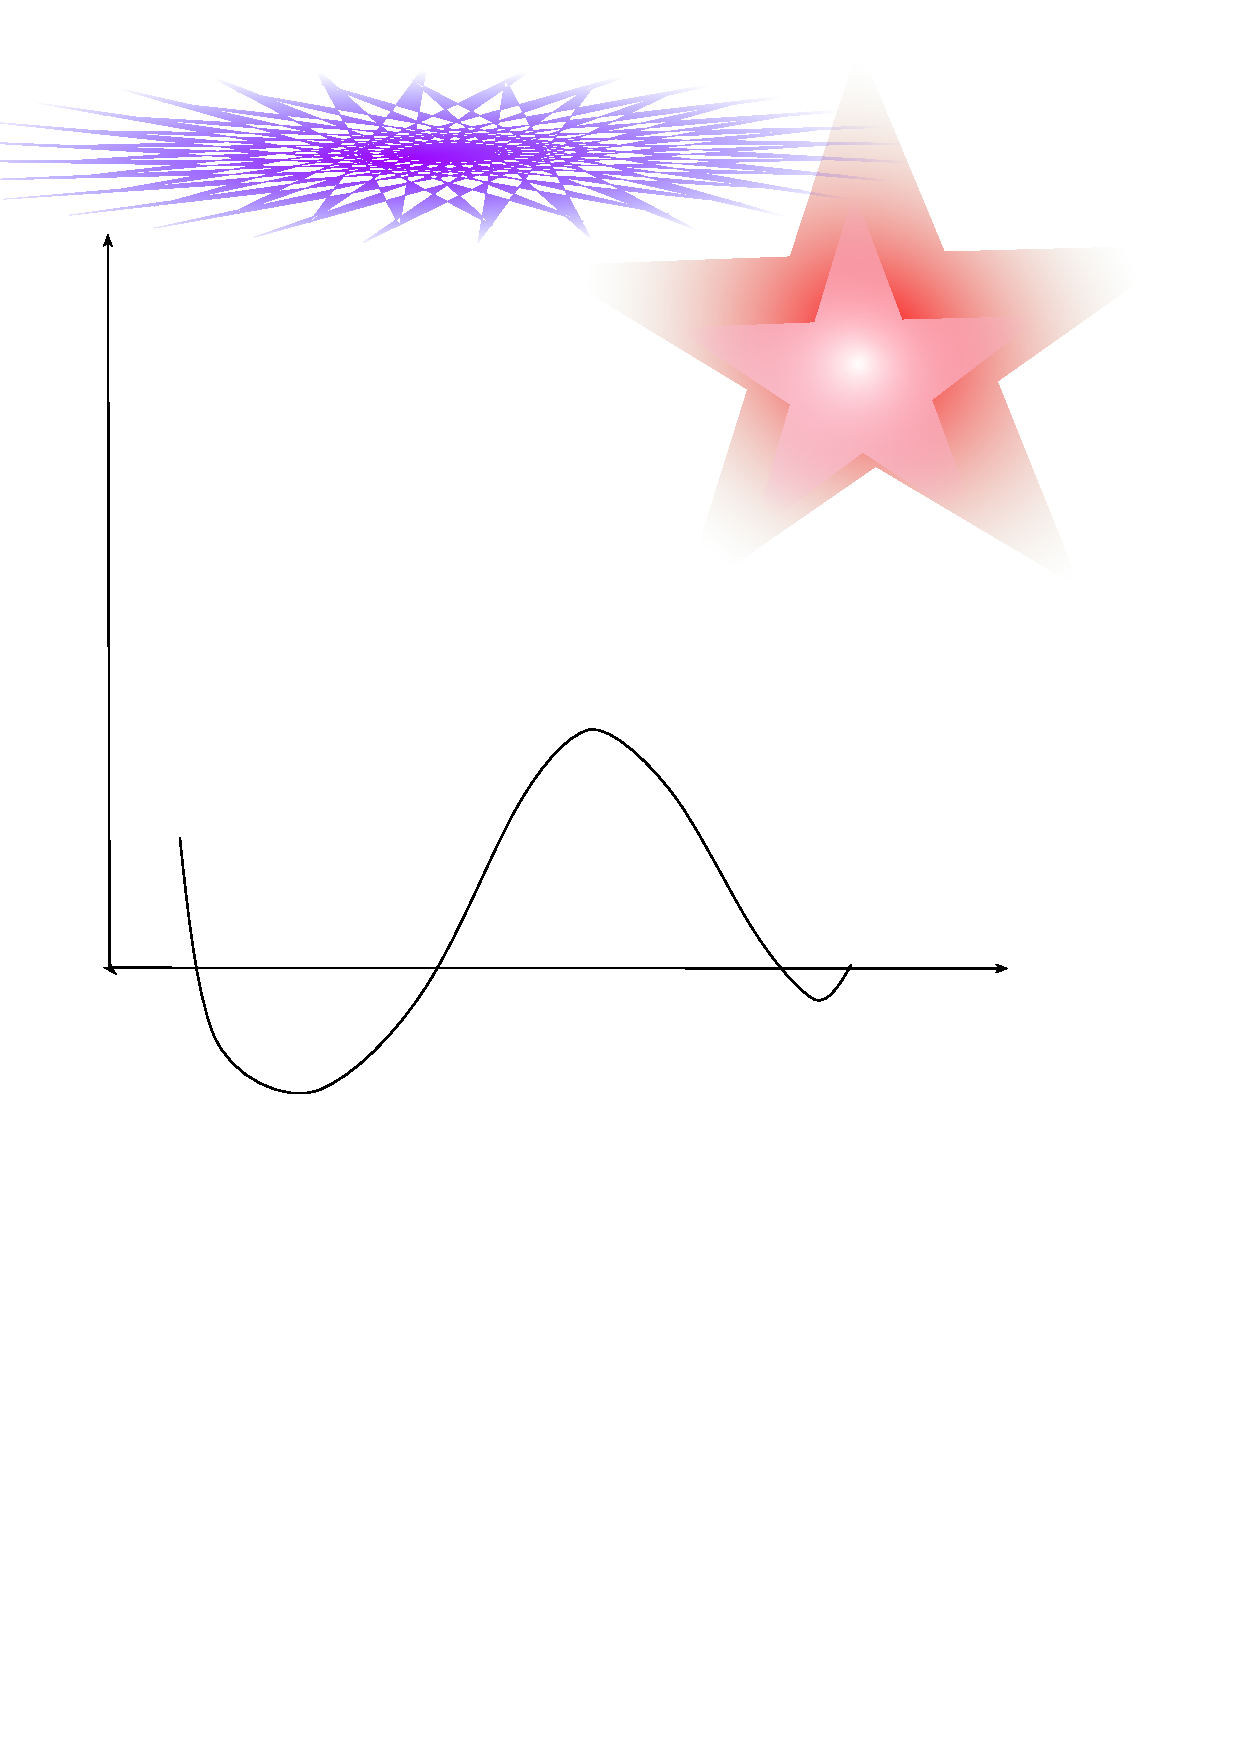
\includegraphics[width=0.8\textwidth]{misc}
  \caption{misc}
  \label{fig:misc}
\end{figure}

\end{document}
